%%%%%%%%%%%%%%%%%%%%%%%%%%%%%%%%%%%%%%%%%%%%%%%%%%%%%%%%%%%%%%%%%%%%%%%%%%%%%%%%%
\section{Snakemake Wrappers}
{   
	\usebackgroundtemplate{
		\vbox to \paperheight{\vfil\hbox to \paperwidth{\hfil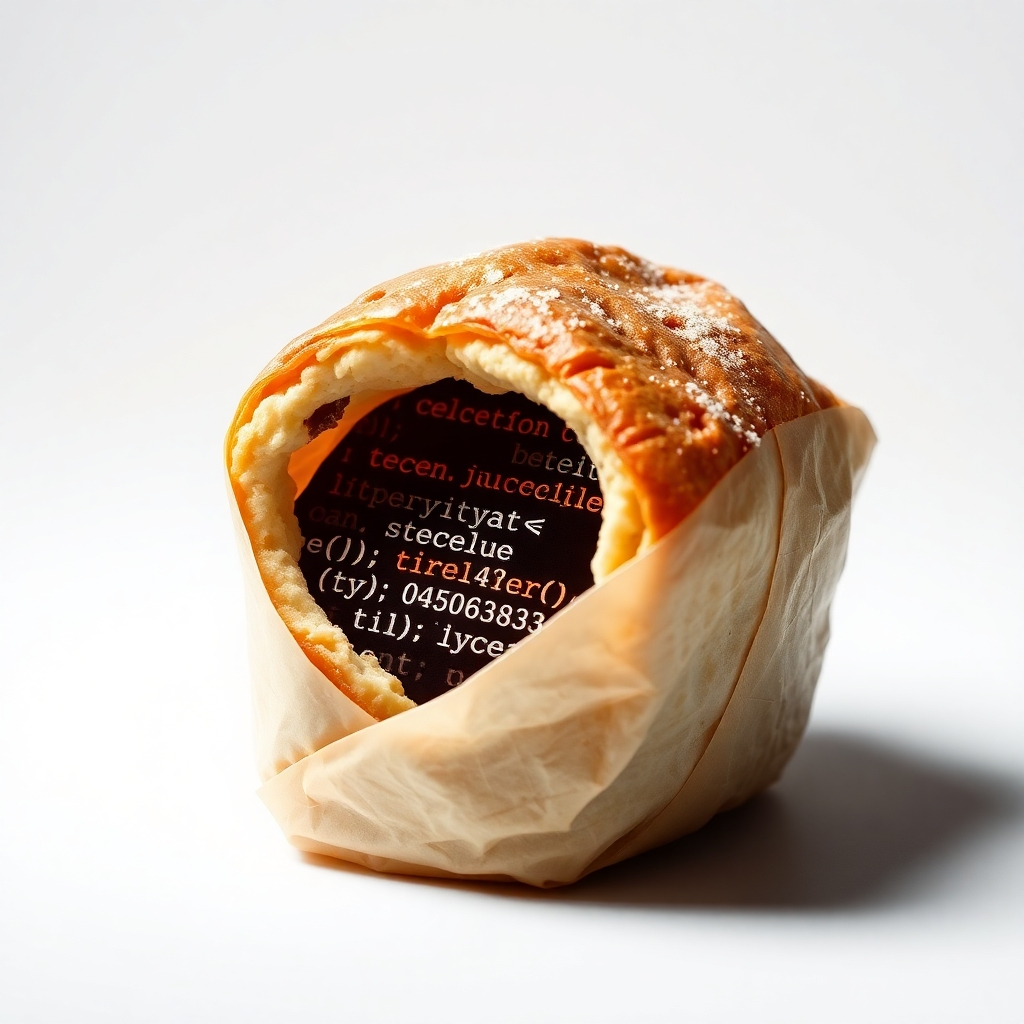
\includegraphics[height=.7\paperheight]{misc/wrapper.jpg}\hfil}\vfil}
	}
	\frame{
		\frametitle{Using \Snakemake-Wrappers}
		\begin{mdframed}[tikzsetting={draw=white,fill=white,fill opacity=0.8,
				line width=0pt},backgroundcolor=none,leftmargin=0,
			rightmargin=150,innertopmargin=4pt,roundcorner=10pt]
			\tableofcontents[currentsection,sections={1-4},hideothersubsections]
		\end{mdframed}
	}
}

%%%%%%%%%%%%%%%%%%%%%%%%%%%%%%%%%%%%%%%%%%%%%%%%%%%%%%%%%%%%%%%%%%%%%%%%%%%%%%%%
\subsection{Using Wrappers}

%%%%%%%%%%%%%%%%%%%%%%%%%%%%%%%%%%%%%%%%%%%%%%%%%%%%%%%%%%%%%%%%%%%%%%%%%%%%%%%%
\begin{frame}
    \frametitle{What is this about?}
    \begin{question}[Questions]
        \begin{itemize}
            \item What is a \Snakemake{} Wrapper?
            \item How can \Snakemake{} wrappers be used to write reproducible workflows?
        \end{itemize}
    \end{question}
    \begin{docs}[Objectives]
        \begin{enumerate}
            \item Introduce the concept of \Snakemake{} wrappers
            \item Include \Snakemake{} wrappers in your workflows
            \item Reproducibility of \Snakemake{} wrappers
        \end{enumerate}
    \end{docs}
\end{frame}

%%%%%%%%%%%%%%%%%%%%%%%%%%%%%%%%%%%%%%%%%%%%%%%%%%%%%%%%%%%%%%%%%%%%%%%%%%%%%%%%
\begin{frame}{Introduction to Wrappers}
    For a single tool, \Snakemake{} Wrappers do:
    \begin{itemize}[<+->]
        \item Document usage
        \item Describe the dependencies
        \item Provide a way to call the tool with information from Snakemake
    \end{itemize}
    This setup makes Snakemake wrappers reusable across multiple workflows.
\end{frame}

%%%%%%%%%%%%%%%%%%%%%%%%%%%%%%%%%%%%%%%%%%%%%%%%%%%%%%%%%%%%%%%%%%%%%%%%%%%%%%%%
\begin{frame}{Introduction to Wrappers}
    Wrappers consist of three components:
    \begin{enumerate}
        \item A description of their usage (\altverb{meta.yaml})
        \item A conda environment description of all dependencies of the tool (\altverb{environment.yaml})
        \item A python script that invokes the tool (\altverb{wrapper.py})
    \end{enumerate}
    Since they are reusable, there is a large repository online of tried and tested 
    wrappers written by the community:
    \pause
    \begin{docs}
    	You can browse the \lhref{https://snakemake-wrappers.readthedocs.io}{snakemake-wrapper overview page} to select your desired wrapper. New Wrappers are added frequently.
    \end{docs}
\end{frame}

%%%%%%%%%%%%%%%%%%%%%%%%%%%%%%%%%%%%%%%%%%%%%%%%%%%%%%%%%%%%%%%%%%%%%%%%%%%%%%%%
\begin{frame}[fragile]
	\frametitle{\Interlude{Dealing with multiple Extensions}}
	\begin{warning}
		So far, we were referring to \emph{one} file. But alignment software like \altverb{bwa} requires all those files with multiple extensions! {\bf This is not safe!}
	\end{warning}
    To require multiple extensions \Snakemake provides the \altverb{multiext()}-function:
    \begin{lstlisting}[language=Python,style=Python]
rule bwa_map:
    input:
      ...
      idx=multiext("genome", ".amb", ".fa",
                   ".ann", ".bwt", ".pac", ".sa")
      ...
    \end{lstlisting}
	Now, \emph{all} listed extensions are required to be present for the file with the prefix \altverb{genome}!
\end{frame}



%%%%%%%%%%%%%%%%%%%%%%%%%%%%%%%%%%%%%%%%%%%%%%%%%%%%%%%%%%%%%%%%%%%%%%%%%%%%%%%%
\begin{frame}[fragile]{Using Wrappers - The Example}
	\begin{docs}
		The following example uses the \altverb{bwa-mem} wrapper from the \Snakemake-community wrappers repository. The example is specific and let us illustrate the usage.
		We will cover the usage step by step and specifically:
		\begin{itemize}
			\item How to find a wrapper?
			\item How to use a wrapper.
		\end{itemize}
	\end{docs}
\end{frame}

%%%%%%%%%%%%%%%%%%%%%%%%%%%%%%%%%%%%%%%%%%%%%%%%%%%%%%%%%%%%%%%%%%%%%%%%%%%%%%%%
\begin{frame}[fragile]{Using Wrappers}
    Using \Snakemake{} wrappers ease your life as a workflow programmer:
    \begin{lstlisting}[language=Python,style=Python,basicstyle=\footnotesize]
rule bwa_map:
    input:
        reads=["input/{sample}_1.fq.gz", 
               "input/{sample}_2.fq.gz"],
        idx=multiext("genome", ".amb", 
                 ".ann", ".bwt", ".pac", ".sa"),
    output:
        "output/{sample}.bam"
    params:
        extra=r"-R '@RG\tID:{sample}\tSM:{sample}'",
        sorting="none",  
        sort_order="queryname",  
        sort_extra="", 
    threads: 8
    wrapper:
        "v3.2.0/bio/bwa/mem"
    \end{lstlisting}
\end{frame}

%%%%%%%%%%%%%%%%%%%%%%%%%%%%%%%%%%%%%%%%%%%%%%%%%%%%%%%%%%%%%%%%%%%%%%%%%%%%%%%%
\begin{frame}[fragile]{Using Wrappers: Calling a Wrapper}
	The \altverb{wrapper} directive signals that \Snakemake{} should execute this rule with
	a wrapper.
	\begin{lstlisting}[language=Python,style=Python,basicstyle=\small]
rule bwa_map:
	...
	@wrapper:@
		@"v3.2.0/bio/bwa/mem"@
	\end{lstlisting}
	\begin{docs}
		\begin{columns}
			\begin{column}{0.5\textwidth}
				Here, we instruct the code to run with the \altverb{wrapper}-directive.
				It specifies 
				\begin{itemize}
					\item a version
					\item a directory
					\item and selects a tool.
				\end{itemize}
			\end{column}
			\begin{column}{0.5\textwidth}\pause
				The path to the tool is given relative to the workflow or a path given by the \altverb{--wrapper-prefix}
				flag. By default \Snakemake automatically downloads wrappers from the  \lhref{https://github.com/snakemake/snakemake-wrappers}{wrappers} repository.
		    \end{column}	
		\end{columns}
	\end{docs}
\end{frame}

%%%%%%%%%%%%%%%%%%%%%%%%%%%%%%%%%%%%%%%%%%%%%%%%%%%%%%%%%%%%%%%%%%%%%%%%%%%%%%%%
\begin{frame}[fragile]{Using Wrappers: In- and Output}
    \altverb{input} and \altverb{output} of the rules has to match the definition of the wrapper:
    \begin{lstlisting}[language=Python,style=Python,basicstyle=\tiny]
rule bwa_map:
    input:
        reads=["input/{sample}_1.fq.gz", 
               "input/{sample}_2.fq.gz"],
        idx=multiext("genome", ".amb", ".ann", 
                     ".bwt", ".pac", ".sa"),
    output:
        "output/{sample}.bam"
    ...
    \end{lstlisting}
    \begin{docs}
        The \altverb{bwa-mem} wrapper expects an input object with two attributes
        \altverb{reads} and \altverb{idx} and writes to a single output file.\newline
        The example builds on short reads (hence: 2 inputs) and the \altverb{multiext}-directive allows samples to have multiple different extensions.
    \end{docs}
\end{frame}

%%%%%%%%%%%%%%%%%%%%%%%%%%%%%%%%%%%%%%%%%%%%%%%%%%%%%%%%%%%%%%%%%%%%%%%%%%%%%%%%
\begin{frame}[fragile]{Using Wrappers: Parameters}
    Parameters may be used by wrappers to influence the behaviour, settings or resource usage.
    \begin{lstlisting}[language=Python,style=Python,basicstyle=\tiny]
rule bwa_map:
    ...
    params:
        extra=r"-R '@RG\tID:{sample}\tSM:{sample}'",
        sorting="none",  # Can be 'none', 'samtools' or 'picard'.
        sort_order="queryname",  # Can be 'queryname' or 'coordinate'.
        sort_extra="",  # Extra args for samtools/picard.
    threads: 8
    ...
    \end{lstlisting}
    \begin{docs}
        \altverb{bwa-mem} supports custom arguments like \altverb{sort_order} and
        the common \altverb{extra} flag, that is used to supply command line parameters
        for the invocation of the tool. The \altverb{threads} and \altverb{resources}
        settings from a Snakemake rule are also commonly used to set memory or parallelization parameters for each tool.
    \end{docs}
\end{frame}
 
 %%%%%%%%%%%%%%%%%%%%%%%%%%%%%%%%%%%%%%%%%%%%%%%%%%%%%%%%%%%%%%%%%%%%%%%%%%%%%%%%
 \begin{frame}{Advantages of Wrappers}
     Using wrappers has many great advantages compared to \altverb{run} or \altverb{shell}:
     \begin{itemize}[<+->]
         \item Code is reusable across workflows and can be shared with others
         \item Complex invocations of tools do not clutter your \Snakemake{} workflow definitions
         \item With versioned wrappers, you workflow is easily reproducible
         \item Community wrappers often get you started quickly using a new tool correctly
     \end{itemize}
 \end{frame}

\setcounter{preframe_handson}{\value{handson}}
%%%%%%%%%%%%%%%%%%%%%%%%%%%%%%%%%%%%%%%%%%%%%%%%%%%%%%%%%%%%%%%%%%%%%%%%%%%%%%%%
\begin{frame}
	\frametitle{\HandsOn{Implement Wrapper Usage}}
	\setcounter{handson}{\value{preframe_handson}}
    Navigate to the wrapper page: \url{https://snakemake-wrappers.readthedocs.io/en/stable/} - you can search for \altverb{snakemake} + \altverb{wrappers}, too.\newline
    \vspace{-0.5em}
    \begin{question}
    	\begin{itemize}[<+->]
    		\item which is a suitable wrapper for our mapping rule?
    		\item Which is a suitable wrapper for the indexing rule?
    		\item Do you think we need to change something?
    	\end{itemize}
    \end{question}
    \vspace{-0.5em}
    \pause\footnotesize
    \begin{docs}[Solution]
    	\begin{itemize}[<+->]
    		\item \altverb{v5.7.0/bio/bwa/mem}
    		\item \altverb{v5.7.0/bio/samtools/index}
    		\item the suffixes for our reference do not match
    		\item we need to select \altverb{sorting="samtools} - why?
    		\item we need to select \altverb{sort_order="coordinate"} - why?
    	\end{itemize}
    \end{docs}
\end{frame}


%%%%%%%%%%%%%%%%%%%%%%%%%%%%%%%%%%%%%%%%%%%%%%%%%%%%%%%%%%%%%%%%%%%%%%%%%%%%%%%%
\begin{frame}
	\frametitle{\HandsOn{Implement Wrapper Usage II}}
	\setcounter{handson}{\value{preframe_handson}}
	Replace the rules \altverb{bwa_map} and \altverb{samtools_index} with wrapper rules.
	\begin{hint}
		Remember
		\begin{itemize}
			\item Take the example code from the wrappers web page.
			\item for bwa and sorting we use: \altverb{v5.7.0/bio/bwa/mem}
			\item for the indexing we use \altverb{v5.7.0/bio/samtools/index}
			\item the suffixes for our reference do not match, enter the appropriate ones
			\item we need to select \altverb{sorting="samtools} and
			\item \altverb{sort_order="coordinate"} for the wrapper based \altverb{bwa_map} rule.
		\end{itemize}
	\end{hint}
    
    \begin{task}
    	Try it!
    \end{task}
\end{frame}

%%%%%%%%%%%%%%%%%%%%%%%%%%%%%%%%%%%%%%%%%%%%%%%%%%%%%%%%%%%%%%%%%%%%%%%%%%%%%%%%
\begin{frame}
  \frametitle{Solution to the Wrapper Exercise}
  A solution is in \altverb{<++course.pathtosolutions++>/13_Snakefile_wrapper}.
\end{frame}
